\subsection{Base de Datos SQLite}

\par \noindent
La base de datos SQLite definida en la sección es donde se guardan todas las medidas de temperatura realizadas por el prototipo. El hecho de ser un fichero en el teléfono lo hace versátil y eficiente para una base de datos local. 


\par \noindent
Por base de datos local hacemos entender que la información se mantendrá en la memoria del teléfono que se esté utilizando. SQLite se basa en una base de datos SQL; por lo que, implementó una base de datos relacional. 

\begin{figure}[H]
	\centering
	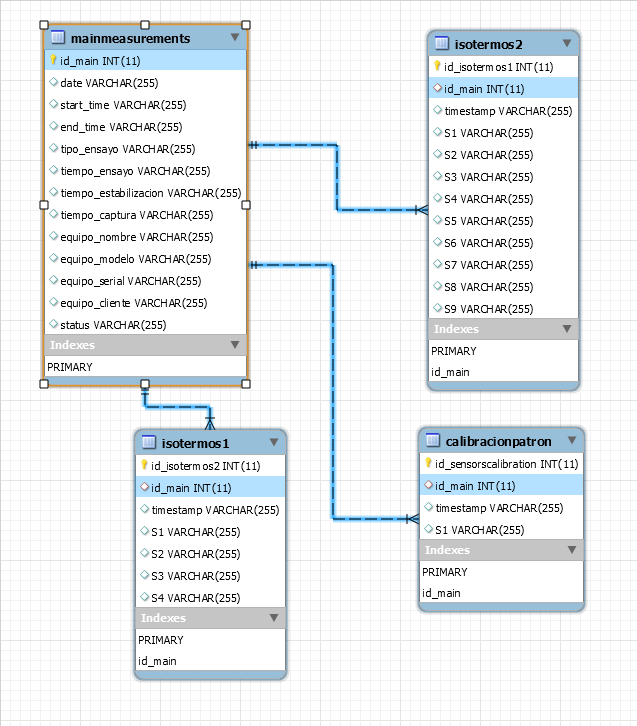
\includegraphics[width=0.8\linewidth]{db1.png}
	\caption{Estructura de la Base de Datos}
\end{figure}

\clearpage

\par \noindent
La tabla principal es "mainmeasurements" donde se toman los datos del equipo y parámetros del ensayo. Mientras que las otras tablas con los nombres de los tipos de ensayo son donde se guardan las medidas de temperatura. Estas tablas están relacionadas a la tabla principal, pero no entre ellas.


\par \noindent
Hasta el momento ha cubierto el desarrollo del firmware del dispositivo, el código que maneja el prototipo. La aplicación en Android la cual guarda la información de temperaturas. El último punto por cubrir es el armazón del arquetipo. Hasta ahora solo se ha visto la placa del circuito. Pero primero se diseño un modelo tridimensional y luego se imprimió utilizando una impresora 3D.

